\documentclass[a4paper, 11pt,reqno]{article}
\input{/Users/olivierglorieux/Desktop/BCPST/2020:2021/preambule.tex}
\usepackage{enumitem}

\newif\ifshow
\showtrue
\input{/Users/olivierglorieux/Desktop/BCPST/2021:2022/ifshow.tex}

\author{Olivier Glorieux}


\begin{document}

\title{Correction DS 1 
}


\begin{exercice}
Résoudre pour $x \in \R$ l'inéquation $$\frac{1}{x+1}\leq \frac{x}{x+2}. \quad (I)$$

Ecrire un script Python, qui demande à l'utilisateur un nombre flottant $x$ et qui affiche  True si $x$ vérifie l'équation $(I)$ et False sinon. 
\end{exercice}
\vspace{1cm}

\begin{exercice}
On considère l'équation suivante d'inconnue $x\in \R : $ 
$$\floor{2x-\sqrt{5x-1}} =0 \quad \quad (E)$$
\begin{enumerate}
\item Déterminer le domaine de définition de $(E)$. 
\item Dire si les réels suivants sont solutions ou non de $(E)$
$$x_1 = \frac{1}{5}, \, x_2 = \frac{1}{2}, \, x_3 =1,\, x_4=12$$
\item Pour tout $a\in \R$, rappeler  un encadrement de la partie entière de $a$ en fonction de $a$. 
\item Montrer que résoudre $(E)$ est équivalent à résoudre le système :
$$\left\{\begin{array}{clc}
\sqrt{5x-1} >&2x-1 &\quad(E_1)\\ 
\sqrt{5x-1} \leq &2x&\quad(E_2)
\end{array}\right.
$$
\item Résoudre les deux inéquations obtenues à la question précédente. 
\item Résoudre $(E)$. 
\end{enumerate}
\end{exercice}

\begin{correction}
\begin{enumerate}
\item Seule la fonction $x\mapsto \sqrt{x}$ n'est pas définie sur $\R$ mais sur $\R_+$ ainsi $(E)$ est bien définie pour tout $x$ tel que $5x-1\geq 0$ c'est-à-dire 
\conclusion{ $D_E=]\frac{1}{5},+\infty[$}
\item Cours 
\conclusion{$\forall a\in \R\, \quad  a-1 <\floor{a}\leq a$}

\item Notons $f(x) = \floor{2x-\sqrt{5x-1} }$ 
On a $f(\frac{1}{5}) = \floor{2\frac{1}{5}-\sqrt{5\frac{1}{5}-1} }= \floor{2\frac{1}{5}} =0$
Donc \conclusion{$\frac{1}{5}$ est solution de $E$}

On a $f(\frac{1}{2} )  =\floor{2\frac{1}{2}-\sqrt{5\frac{1}{2}-1} } = \floor{1-\sqrt{\frac{3}{2} }}$ Or $\frac{3}{2}> 1 $ donc 
$\sqrt{\frac{3}{2}} >\sqrt{1}=1$ et donc 
$1-\sqrt{\frac{3}{2} }<0$ ainsi  
\conclusion{$\frac{1}{2}$ n'est pas solution de $E$}

On a $f(1) = \floor{2\times 1-\sqrt{5-1}} =\floor{2-2}=\floor{0}$
\conclusion{$1$ est solution de $E$}

On  a $f(12) = \floor{2\times 12-\sqrt{60-1}}=\floor{24-\sqrt{59}}$ 
Or$ 59<64=8^2$ donc  $\sqrt{59} < 8 $ et 
$24-\sqrt{59}> 24-8=16$ ainsi $f(2)>16 $ et 
\conclusion{$12$ n'est pas solution de $E$}


\item D'après ce qu'on vient de voir, pour tout $x\in D_E$ on a :
$$2x-\sqrt{5x-1} -1<\floor{2x-\sqrt{5x-1} } \leq 2x-\sqrt{5x-1} $$
Si $x$ est solution de $(E)$ on a $\floor{2x-\sqrt{5x-1} }=0$ et donc l'équation $(E)$ équivaut à $2x-\sqrt{5x-1} -1<0 \leq 2x-\sqrt{5x-1} $, soit 
\conclusion{$\left\{\begin{array}{clc}
\sqrt{5x-1} >&2x-1 &\quad(E_1)\\ 
\sqrt{5x-1} \leq &2x&\quad(E_2)
\end{array}\right.
$}

\item Résolvons ces deux inéquations. Tout d'abord la première :
$$\sqrt{5x-1} >2x-1 \quad(E_1)$$
On distingue deux cas : 
\begin{itemize}
\item[$\blacktriangleright$] \underline{Cas 1 :} $2x-1\geq 0$ c'est-à-dire $x\geq \frac{1}{2}$

Alors on peut passer au carré dans l'équation car les deux cotés sont du même signe. On a alors : 
\begin{align*}
(E_1)& \equivaut 5x-1 > (2x-1) ^2\\
& \equivaut 5x-1 > 4x^2-4x+1\\
& \equivaut 4x^2-9x+2<0
\end{align*}
Un petit discriminant comme on aime : 
$\Delta = 9^2 - 4*4*2 = 81- 32= 49 =7^2$. 
$4x^2-9x+2$ admet donc deux racines 
$$r_1 = \frac{9+7}{8}=2 \quadet r_2 =\frac{9-7}{8} = \frac{1}{4}$$

Ainsi les solutions de $(E_1) $ sur $[\frac{1}{2},+\infty[$ sont
\begin{align*}
\cS_1 &= ]\frac{1}{4},2[ \cap [\frac{1}{2},+\infty[ \cap D_E\\
		 &= [\frac{1}{2},2[	
\end{align*}


\conclusion{  Les solutions de $(E_1) $ sur $[\frac{1}{2},+\infty[$ sont  $\cS_1 = [\frac{1}{2},2[	$}

\item[$\blacktriangleright$] \underline{Cas 2 :} $2x-1<0$ c'est-à-dire $x<\frac{1}{2}$

Dans ce cas, tous les réels $x\in D_E$ sont solutions car le membre de gauche est positif et celui de droite négatif. 

\conclusion{  Les solutions de $(E_1) $ sur $]-\infty,\frac{1}{2}[$ sont  $\cS_1' = [\frac{1}{5},\frac{1}{2}]	$}

En conclusion :
\conclusion{  Les solutions de $(E_1) $ sur $D_E$ sont  $\cS = \cS_1\cup \cS_1' = [\frac{1}{5},2[	$}



\end{itemize}

On fait la même chose pour $(E_2) $ 
$$\sqrt{5x-1} \leq 2x \quad(E_2)$$

On distingue deux cas : 
\begin{itemize}
\item[$\blacktriangleright$] \underline{Cas 1 :} $2x\geq 0$ c'est-à-dire $x\geq 0$

Alors on peut passer au carré dans l'équation car les deux cotés sont du même signe. On a alors : 
\begin{align*}
(E_1)& \equivaut 5x-1 \leq  (2x) ^2\\
& \equivaut 5x-1 \leq 4x^2\\
& \equivaut 4x^2-5x+1\geq 0
\end{align*}
Un petit discriminant comme on aime : 
$\Delta = 5^2 - 4*4*1 = 25- 16= 9 =3^2$. 
$4x^2-5x+1$ admet donc deux racines 
$$r_1 = \frac{5+3}{8}=1 \quadet r_2 =\frac{5-3}{8} = \frac{1}{4}$$

Ainsi les solutions de $(E_2) $ sur $[0,+\infty[$ sont
\begin{align*}
\cE_2 &=( ]-\infty, \frac{1}{4}] \cup [1,+\infty[) \cap [0,+\infty[ \cap D_E\\
		 &= [\frac{1}{5} ,\frac{1}{4}] \cup[1,+\infty[	
\end{align*}


\conclusion{  Les solutions de $(E_2) $ sur $[0,+\infty[$ sont  $\cE_2 =  [\frac{1}{5} ,\frac{1}{4}] \cup[1,+\infty[	$}

\item[$\blacktriangleright$] \underline{Cas 2 :} $2x<0$ c'est-à-dire $x<0$

Dans ce cas, aucun réel n'est solution car le membre de gauche est positif et celui de droite négatif. 

\conclusion{  Les solutions de $(E_2) $ sur $]-\infty,0[$ sont  $\cE_2' =\emptyset$}

En conclusion :
\conclusion{  Les solutions de $(E_2) $ sur $D_E$ sont  $\cE = \cE_2\cup \cE_2' =  [\frac{1}{5} ,\frac{1}{4}] \cup[1,+\infty[		$}



\end{itemize}

\item $x$ est solution de $(E)$ si et seulement si il est solution de $(E_1) $ et $(E_2)$, l'ensemble des solutions correspond donc à l'intersection : $\cE \cap \cS =   ([\frac{1}{5} ,\frac{1}{4}] \cup[1,+\infty[	) \cap[\frac{1}{5},2[ = 
[\frac{1}{5} ,\frac{1}{4}] \cup[1,2[$ 

\conclusion{ Les solutions de $(E)$ sont $[\frac{1}{5} ,\frac{1}{4}] \cup[1,2[$ }


\end{enumerate}
\end{correction}








\begin{exercice}
Soit $f$ la fonction définie par :
$$f : x\mapsto \frac{e^{2x} -1}{e^{2x}+1}$$
\begin{enumerate}
\item Etudier la parité de $f$. 
\item Donner les limites de $f$  en $+\infty $ et $-\infty$. 
\item Dresser le tableau de variations de $f$ 
%\item Montrer que pour tout $x\in \R$, $f'(x) =1-f^2(x)$.
\end{enumerate}
\end{exercice}
\vspace{1cm}











\begin{exercice}
On considère les nombres réels $\alpha =\sqrt[3]{2+\sqrt{5}}$ et $\beta =\sqrt[3]{2-\sqrt{5}}$. On rappelle que pour tout réel $y$ on note $\sqrt[3]{y}$ l'unique solution de l'équation $x^3=y$ d'inconnue $x$.

Le but de l'exercice est de donner des expressions simplifiées de $\alpha$ et $\beta$. 

\begin{enumerate}
\item Ecrire un script Python qui permet d'afficher une valeur approchée de $\alpha$.
\item 
\begin{enumerate}
\item Calculer $\alpha \beta$ et $\alpha^3+\beta^3$.
\item Vérifier que $\forall (a,b)\in \R^2$, $(a+b) ^3 = a^3 +3a^2b+3ab^2 +b^3$.
\item En déduire que  $(\alpha+\beta)^3= 4-3(\alpha+\beta)$ 
\end{enumerate}
\item On pose $u=\alpha +\beta$ et on considère la fonction polynomiale $P : x\mapsto x^3+3x-4$. 
\begin{enumerate}
\item A l'aide de  la question précédente montrer que $u$ est une racine de $P$ c'est-à-dire que $P(u)=0$. 
\item Trouver une autre racine \og évidente \fg\, de $P$.
\item Trouver trois nombres réels $a$, $b$, et $c$ tels que $\forall x\in \R, P(x) = (x-1)(ax^2+bx+c)$
\item Résoudre l'équation $P(x)=0$ pour $x\in \R$.
\item En déduire la valeur de $u$. 
\end{enumerate}
\item On considère la fonction polynomiale $Q : x\mapsto Q(x) = (x-\alpha)(x-\beta)$
\begin{enumerate}
\item A l'aide des questions précédentes, développer et simplifier $Q(x)$ pour tout nombre réel $x$. 
\item En déduire des expressions plus simples de $\alpha $ et $\beta$. 
\end{enumerate}
\end{enumerate}
\end{exercice}

\begin{correction}
\begin{enumerate}
\item \begin{lstlisting}
print((2+5**(1/2))**(1/3))
\end{lstlisting}
\item \begin{enumerate}
\item \begin{align*}
\alpha \beta &= \sqrt[3]{2+\sqrt{5}}\sqrt[3]{2-\sqrt{5}}\\
					&=\sqrt[3]{(2+\sqrt{5})(2-\sqrt{5}}\\
					&=\sqrt[3]{4-5}\\
					&=\sqrt[3]{-1}\\					
					&=-1
\end{align*}

\begin{align*}
\alpha^3+\beta^3&= 2+\sqrt{5}+2-\sqrt{5}\\
							&=4
\end{align*}

\conclusion{$\alpha\beta =-1$ et $\alpha^3+\beta^3=4$}

\item 
\begin{align*}
(a+b)^3&=(a+b)^2(a+b)\\
			&=(a^2+2ab+b^2)(a+b)\\
			&=a^3+2a^2b+ab^2+ba^2+2ab^2+b^3\\
			&=a^3+3a^2b+3ab^2+b^3
\end{align*}

\conclusion{ $\forall (a,b)\in \R^2$, $(a+b) ^3 = a^3 +3a^2b+3ab^2 +b^3$.}
\item 
\begin{align*}
(\alpha+\beta)^3& = \alpha^3 +3\alpha^2\beta +3\alpha \beta^2 +\beta^3\\
&=\alpha^3  +\beta^3 +3\alpha\beta(\alpha + \beta)\\
&=4-3\alpha\beta
\end{align*}
\end{enumerate}
\item 
\begin{align*}
P(u) &= P(\alpha+\beta) \\
	&= (\alpha+\beta)^3+3\alpha\beta -4\\
	&=0 \quad \text{ d'après la question précédente}
\end{align*}

\conclusion{ $u$ est racine de $P$}

\item $1$ est aussi racine de $P$, en effet : $P(1) =1+3-4=0$

\conclusion{ $1$ est racine de $P$}

\item Développons 
$(x-1) (ax^2+bx+c)$ on obtient 
$$(x-1) (ax^2+bx+c) =ax^3 +(b-a)x^2 +(c-b)x -c$$
En identifiant avec $P$, on a : 
$a=1, b-a=0, c-b=3, -c=-4$
c'est à dire 
\conclusion{ $a=1$, $b=1$ et $c=4$}  


\item D'après la question précédente $P(x) =(x-1) (x^2+x+4)$
Le discriminant de $x^2+x+4$ est $\Delta =1-4*4 =-15<0$ 
$x^2+x+4>0$ pour tout $x\in \R$. Ainsi $P(x)=0$ admet pour unique solution 
\conclusion{ $\cS=\{1\}$} 
 
 \item $1$ est racine de $P$, c'est la seule. Comme $u$ est aussi racine, 
 \conclusion{$u=1$ }

\item 
\begin{enumerate}
\item Développons $Q$:
\begin{align*}
Q(x) &= (x-\alpha) (x-\beta)\\
		&=x^2 -(\alpha+\beta)x +\alpha\beta\\
		&=x^2 -x -1
\end{align*}

\conclusion{ Pour tout $x\in \R, \, Q(x) =x^2-x-1$}

\item L'expression $Q(x) = (x-\alpha) (x-\beta)$ montre que les racines de $Q$ sont   $\alpha$ et $\beta$. 

D'autre part, on connait une autre expression des racines de $Q$ à l'aide du discriminant $\Delta =1+4=5$, les racines de $Q$ sont 
$$r_1 = \frac{1+\sqrt{5}}{2}\quadet r_1 = \frac{1-\sqrt{5}}{2}$$

Remarquons que $r_1<r_2$ et on  a $\alpha<\beta$ donc 
\conclusion{ $\alpha =  \frac{1+\sqrt{5}}{2} $ et $\beta =  \frac{1-\sqrt{5}}{2} $ }


\end{enumerate}
\end{enumerate}
\end{correction}










\begin{correction}
L'équation $(I)$ est définie pour tout $x\in D=\R\setminus\{ -2,-1\}$ et pour tout $x\in D$ on a :
\begin{align*}
(I)\equivaut &\frac{1}{x+1}- \frac{x}{x+2}\leq 0\\
\equivaut & \frac{x+2 -x(x+1)}{(x+1)(x+2)}\leq 0\\
\equivaut &  \frac{-x^2 +2 }{(x+1)(x+2)}\leq 0\\
\equivaut &  \frac{x^2 -2 }{(x+1)(x+2)}\geq 0\\
\equivaut &  \frac{(x -\sqrt{2}) (x+\sqrt{2}) }{(x+1)(x+2)}\geq 0
\end{align*}
On fait un tableau de signe  : 

\begin{tikzpicture}[scale=0.8]
   \tkzTabInit[lgt=4]{$x$ /0.5, $x-\sqrt{2}$ /1, $x+\sqrt{2}$ /1, $ x+1$ /1,$ x+2$ /1,    $\frac{(x -\sqrt{2}) (x+\sqrt{2}) }{(x+1)(x+2)}$ /1.5 } {$-\infty$ , $-2$, $-\sqrt{2}$, $-1$, $\sqrt{2}$, $+\infty$}
   \tkzTabLine{, -, , -,,-,,-,z,+ } 
   \tkzTabLine{, -, , -,z,+,,+,,+ } 
   \tkzTabLine{, -, , -,,-,d,+,,+ } 
   \tkzTabLine{, -, d, +,,+,,+,,+ } 
   \tkzTabLine{, +,d , -,z,+,d,-,z,+ } 
\end{tikzpicture}
Les solutions sont donc 
\conclusion{$\bS = ]-\infty, -2[\cup [-\sqrt{2} ,-1[\cup [\sqrt{2}, +\infty[$}

\begin{lstlisting}
x=float(input('Choisissez un reel x')) 
if 1/(x+1) <= x/(x+2):
  print(True)
else:
  print(False)
\end{lstlisting}
\end{correction}


\begin{correction}
\begin{enumerate}
\item La fonction $f$ est bien définie sur $\R$ et 
pour tout $x\in \R$ on  a :
\begin{align*}
f(-x)&=\frac{e^{-2x}-1}{e^{-2x}+1}\\
		&=\frac{\frac{1}{e^{2x}}-1}{\frac{1}{e^{2x}}+1}\\
		&=\frac{1-e^{2x}}{1+e^{2x}}\\
		&=-f(x)
\end{align*}
\conclusion{La fonction $f$ est donc impaire. }
\item 
\begin{align*}
f(x)& = \frac{e^{2x} (1-e^{-2x}) }{e^{2x} (1+e^{-2x})}\\
&=\frac{ 1-e^{-2x} }{1+e^{-2x}}
\end{align*}
Or $\lim_{x\tv +\infty} e^{-2x}=0$ donc
\conclusion{$\lim_{x\tv+\infty} =1$}

$\lim_{x\tv -\infty} e^{2x}=0$ donc
\conclusion{$\lim_{x\tv-\infty} =-1$}

\item 
$f$ est dérivable sur $\R$ et pour tout $x\in \R$ on a:
\begin{align*}
f'(x) & = \frac{2e^{2x} (e^{2x}+1) - 2e^{2x} (e^{2x}-1) }{ (e^{2x}+1)^2}\\
&=  \frac{4e^{2x}}{ (e^{2x}+1)^2}
\end{align*}
Comme l'exponentielle est  positive sur $\R$, $f$ est strictement croissante sur $\R$ et on a le tableau suivant : 




\end{enumerate}
\end{correction}



\end{document}